\documentclass[12pt]{article}

\usepackage{verbatim}
\usepackage{listings}

\usepackage[a4paper,margin=2cm]{geometry}

\usepackage{amsmath}
\usepackage{amssymb}
\usepackage{mathtools}

\usepackage{booktabs} % For tables
\usepackage[table,xcdraw]{xcolor} % For tables

\usepackage{svg} % for .svg's

\usepackage{parskip}

\usepackage{tikz} % TikZ

\usepackage{enumerate}
\usepackage{enumitem}

\usepackage{nameref}

\usepackage{xcolor}

\usepackage{subfiles}

\definecolor{codegreen}{rgb}{0,0.6,0}
\definecolor{codegray}{rgb}{0.5,0.5,0.5}
\definecolor{codepurple}{rgb}{0.58,0,0.82}
\definecolor{backcolour}{rgb}{0.95,0.95,0.92}

\lstdefinestyle{mystyle}{
    backgroundcolor=\color{backcolour},
    commentstyle=\color{codegreen},
    keywordstyle=\color{magenta},
    numberstyle=\tiny\color{codegray},
    stringstyle=\color{codepurple},
    captionpos=b,
    keepspaces=true,
    numbers=left,
    numbersep=5pt,
    showspaces=false,
    showstringspaces=false,
    showtabs=false,
    tabsize=2,
    columns=flexible,
    breaklines=true
}

\lstset{style=mystyle}

\DeclarePairedDelimiter\abs{\lvert}{\rvert}
\DeclarePairedDelimiter\Abs{\lVert}{\rVert}

\usepackage{fancyhdr}

\pagestyle{fancy}
\lhead{\today}
\chead{Assignment 1\\Business Process Intelligence}
\rhead{Marc Ludevid-Wulf\\Til Mohr\\Simon Michau, 406133}

\setlength{\headheight}{50pt}

\begin{document}

\section*{Question 1}
\subfile{Question_1/question_1.tex}

\section*{Question 2}
\subfile{Question_2/question_2.tex}

\section*{Question 3}
\subfile{Question_3/question_3.tex}

\section*{Question 4}
\subfile{Question_4/question_4.tex}

\section*{Question 5}
\subfile{Question_5/question_5.tex}

\section*{Question 6}
\subfile{Question_6/question_6.tex}

\section*{Appendix}
\subsection*{Question 2(b)1}
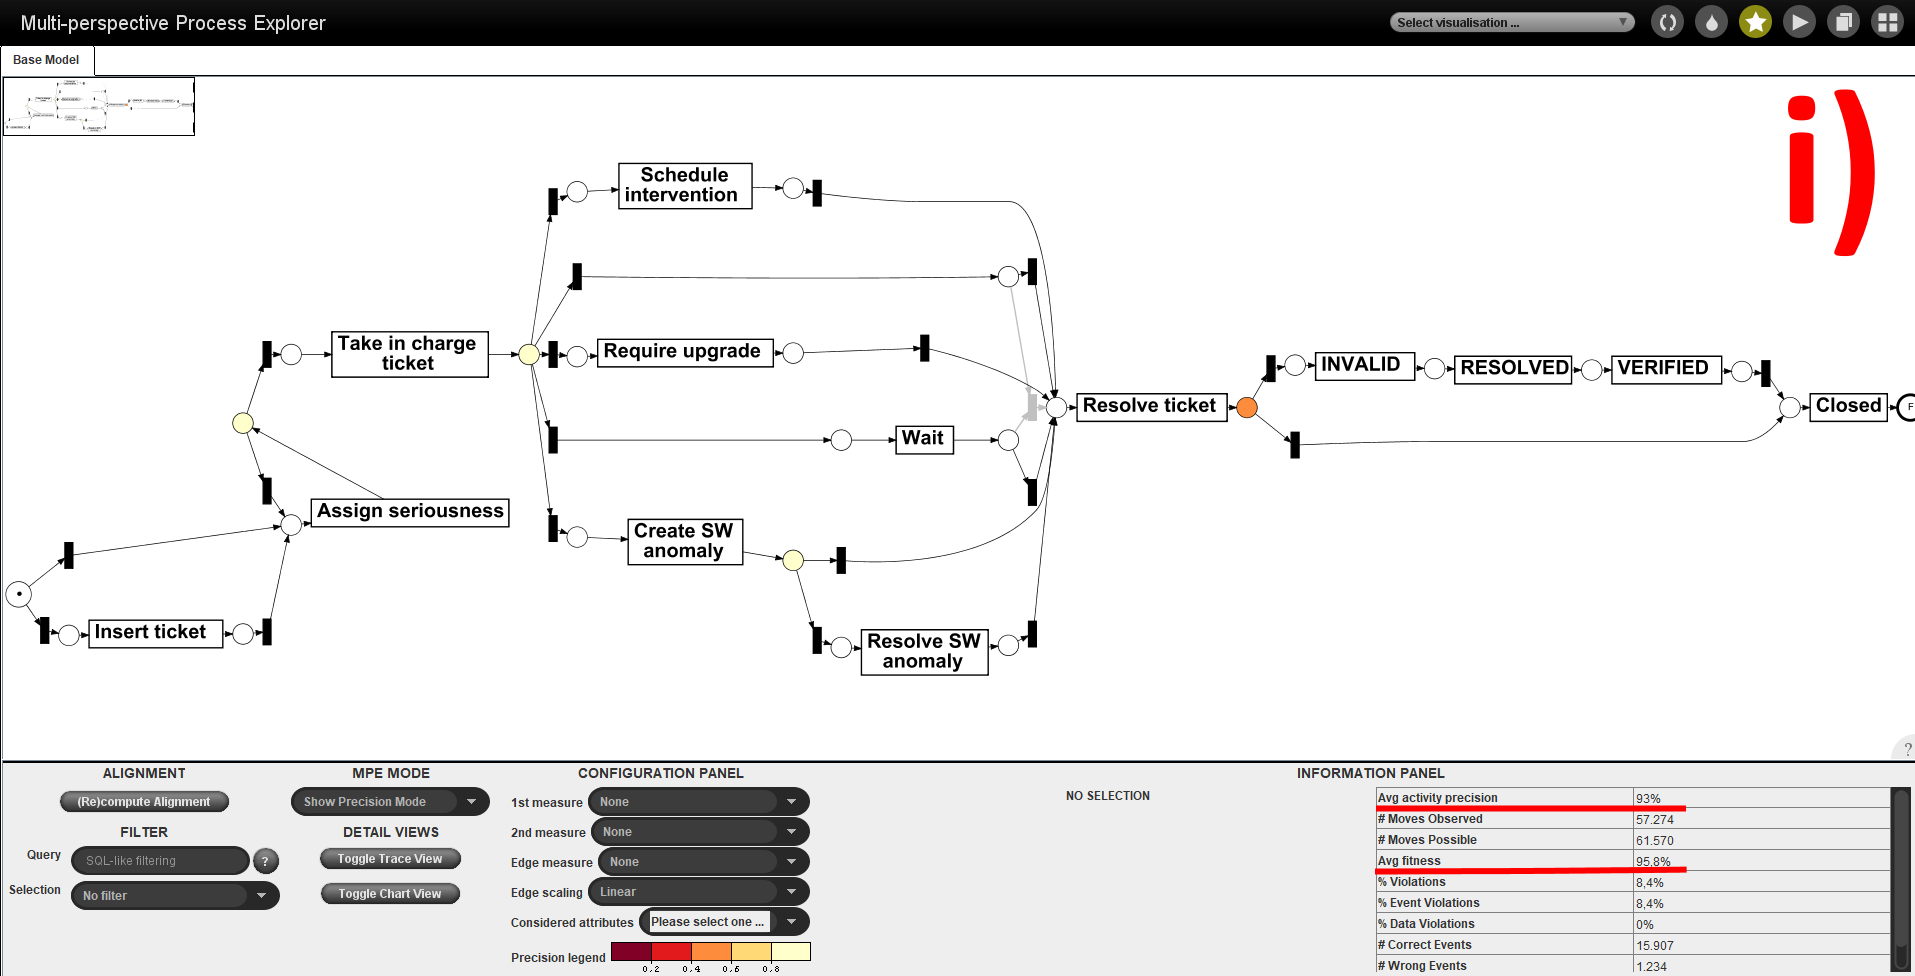
\includegraphics[width=\columnwidth]{Question_2/img/ProM_b_PRE_i.png}\\
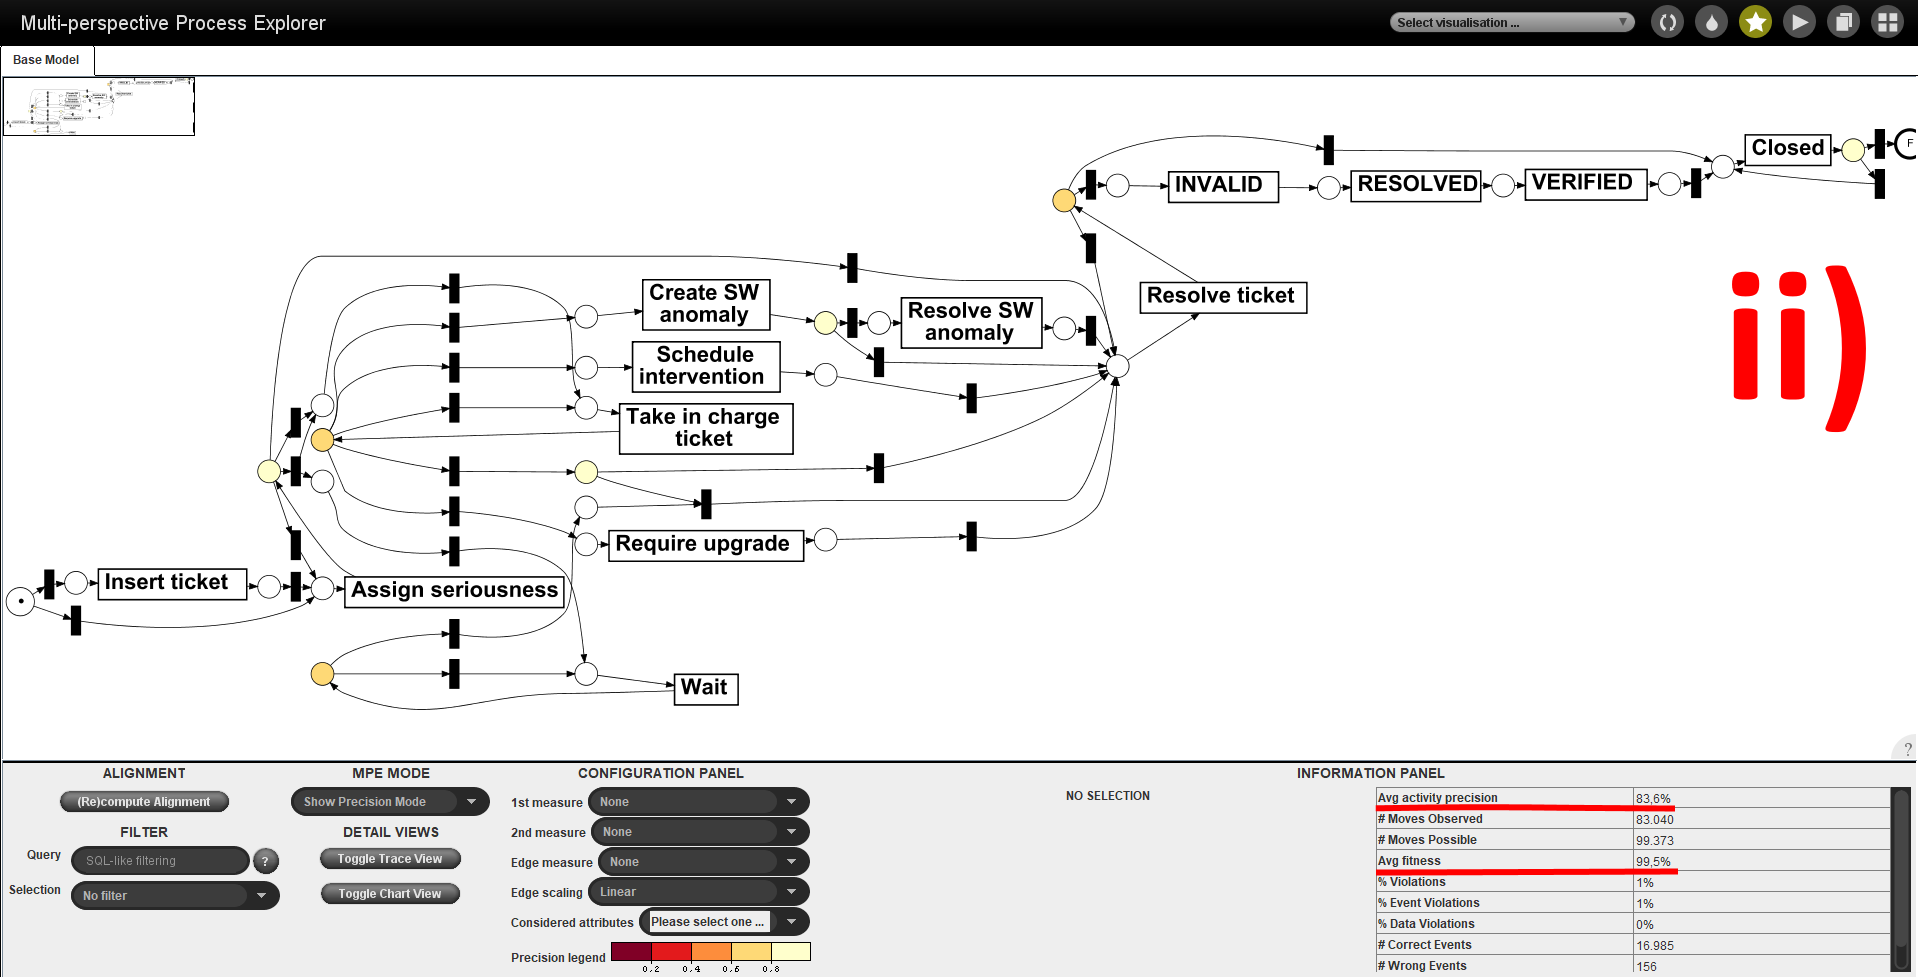
\includegraphics[width=\columnwidth]{Question_2/img/ProM_b_PRE_ii.png}\\
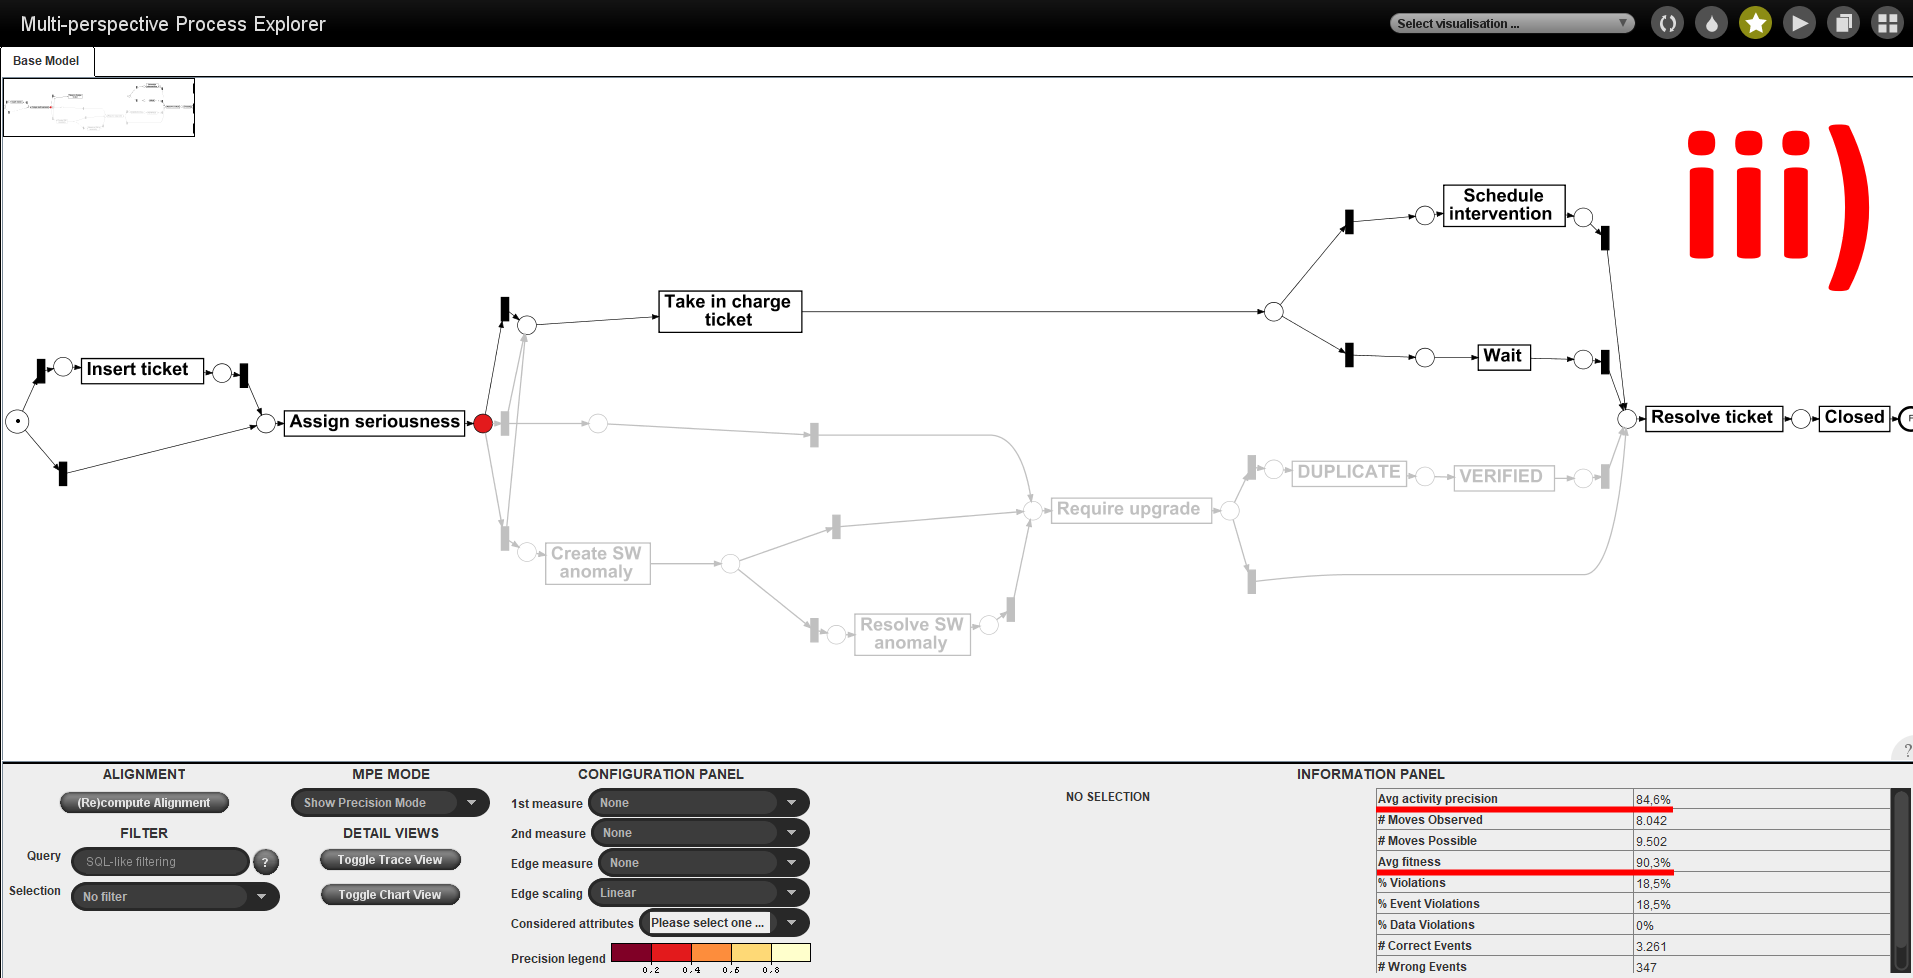
\includegraphics[width=\columnwidth]{Question_2/img/ProM_b_POST_iii.png}\\
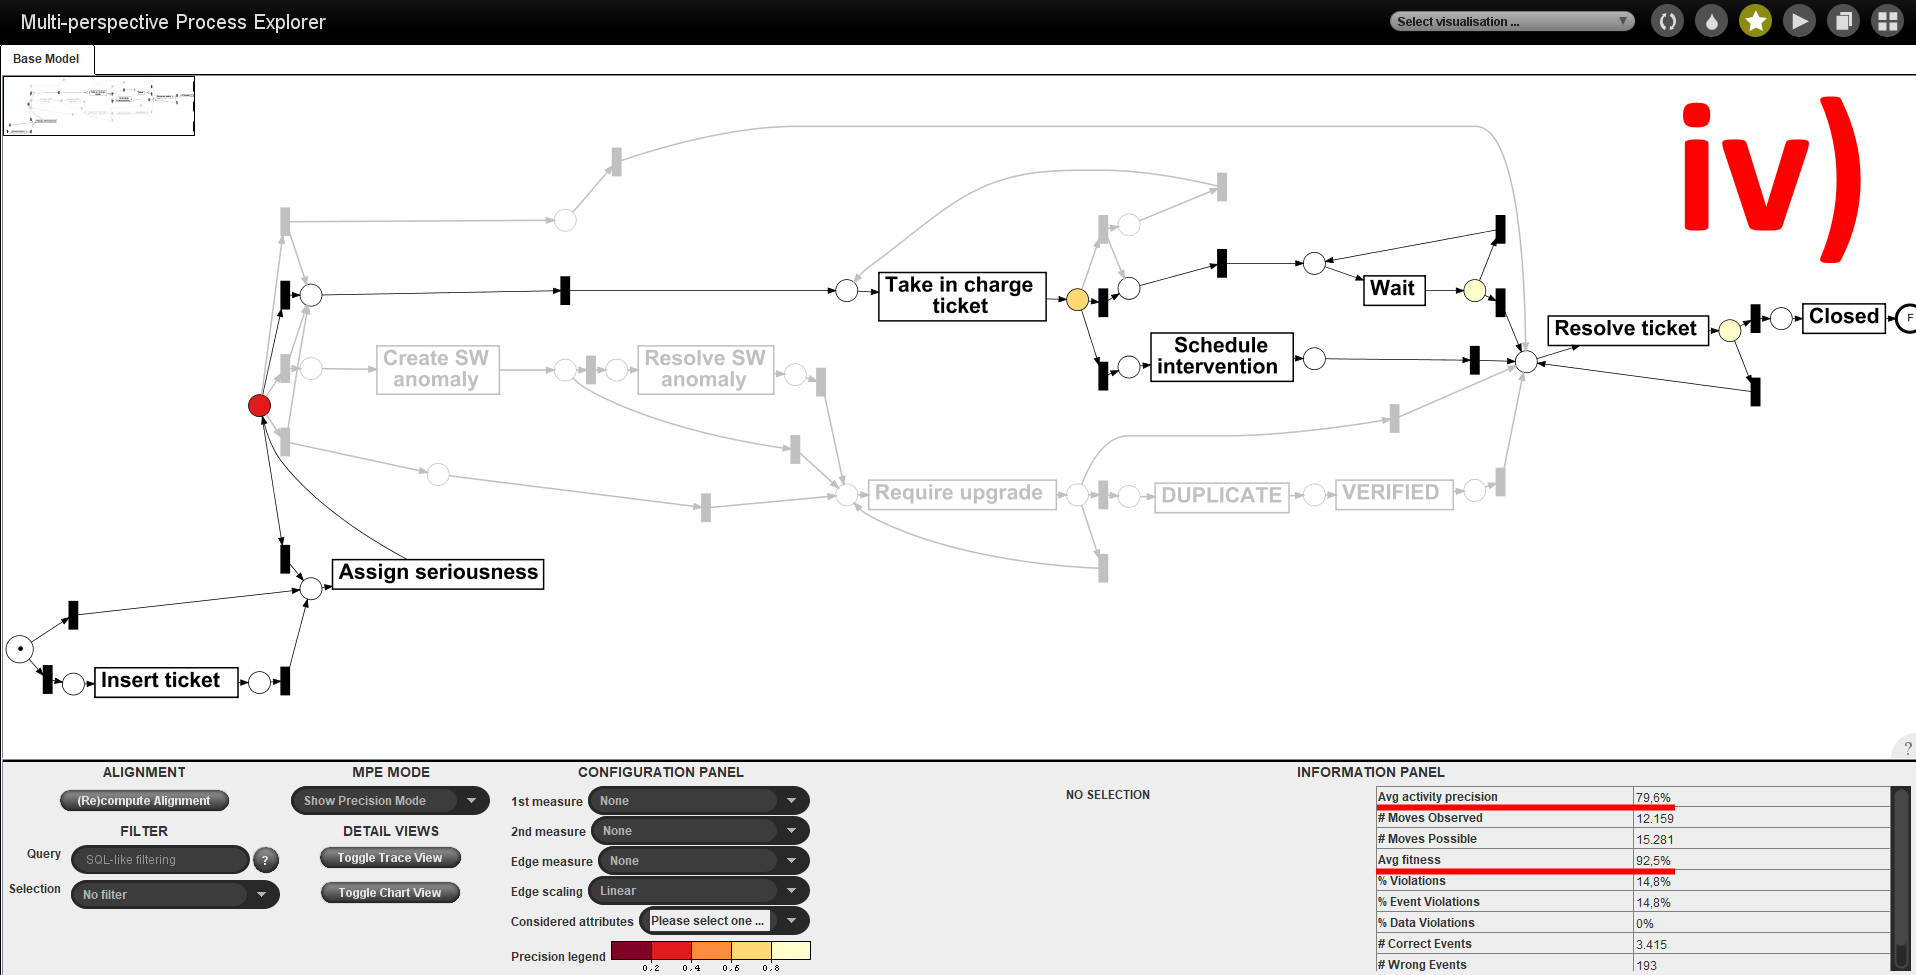
\includegraphics[width=\columnwidth]{Question_2/img/ProM_b_POST_iv.png}\\
\subsection*{Question 2(b)2}
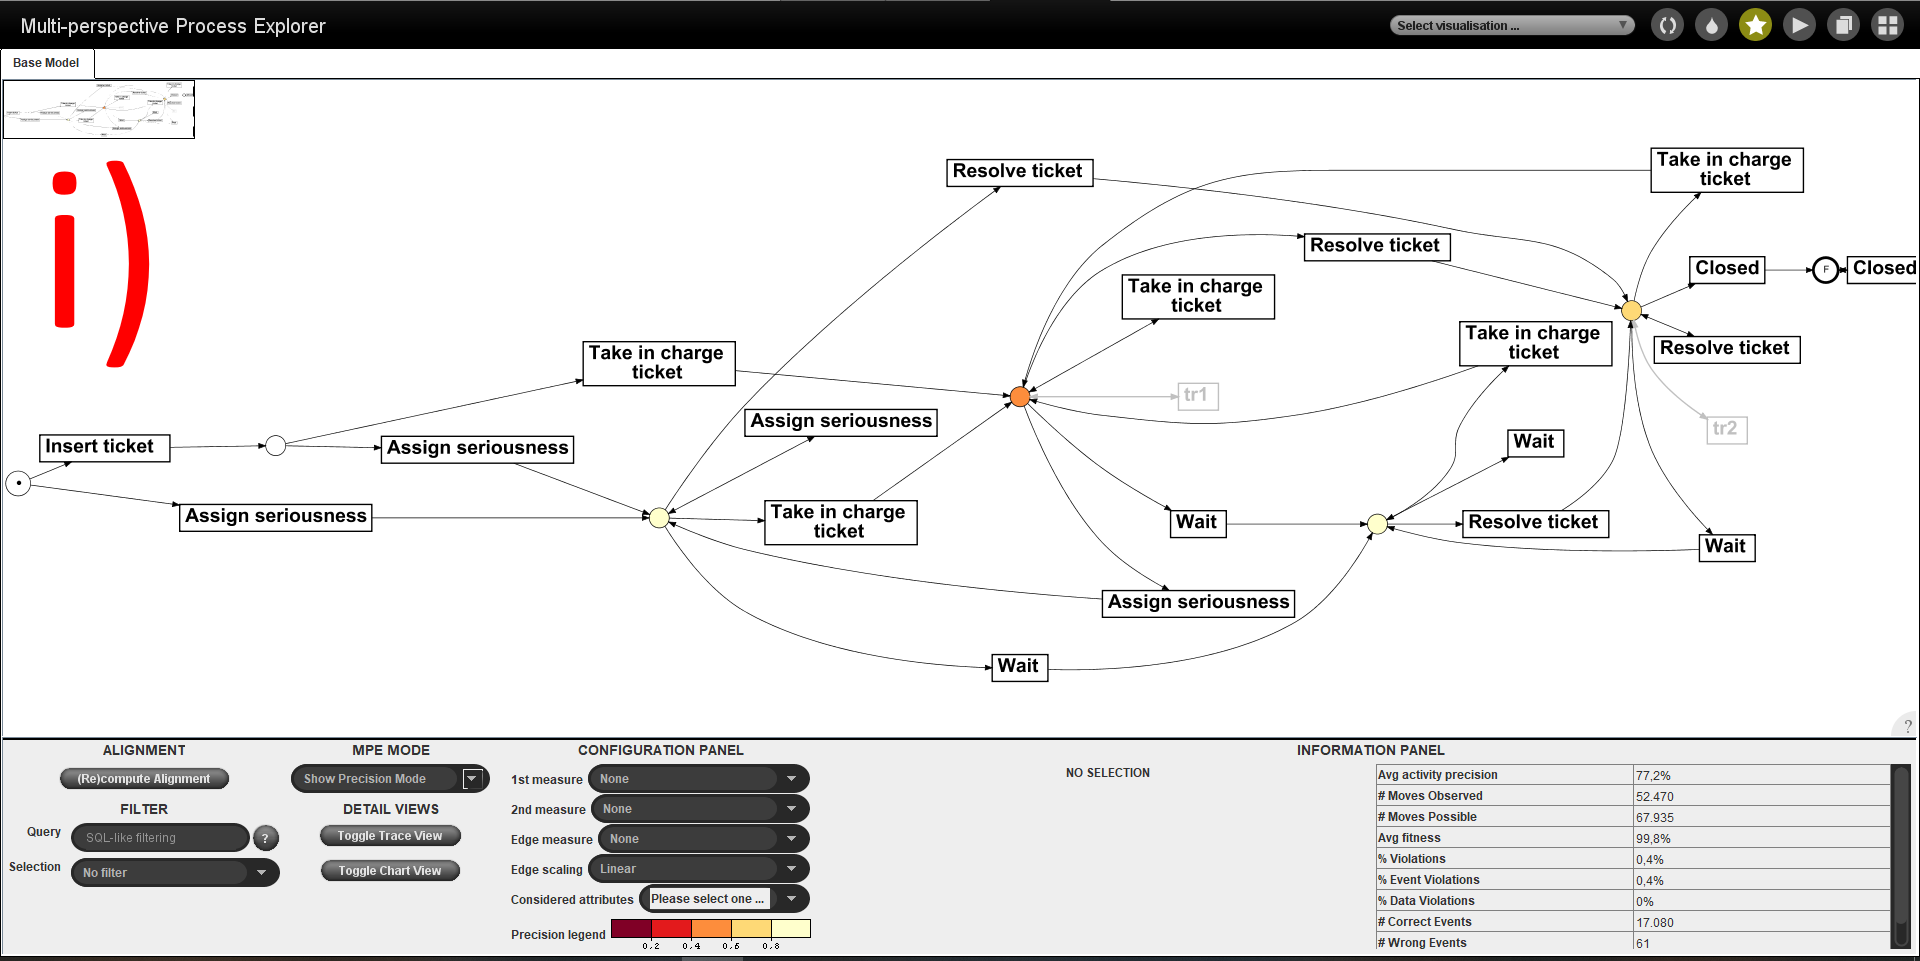
\includegraphics[width=\columnwidth]{Question_2/img/ProM_b_region_i_PRE.png}\\
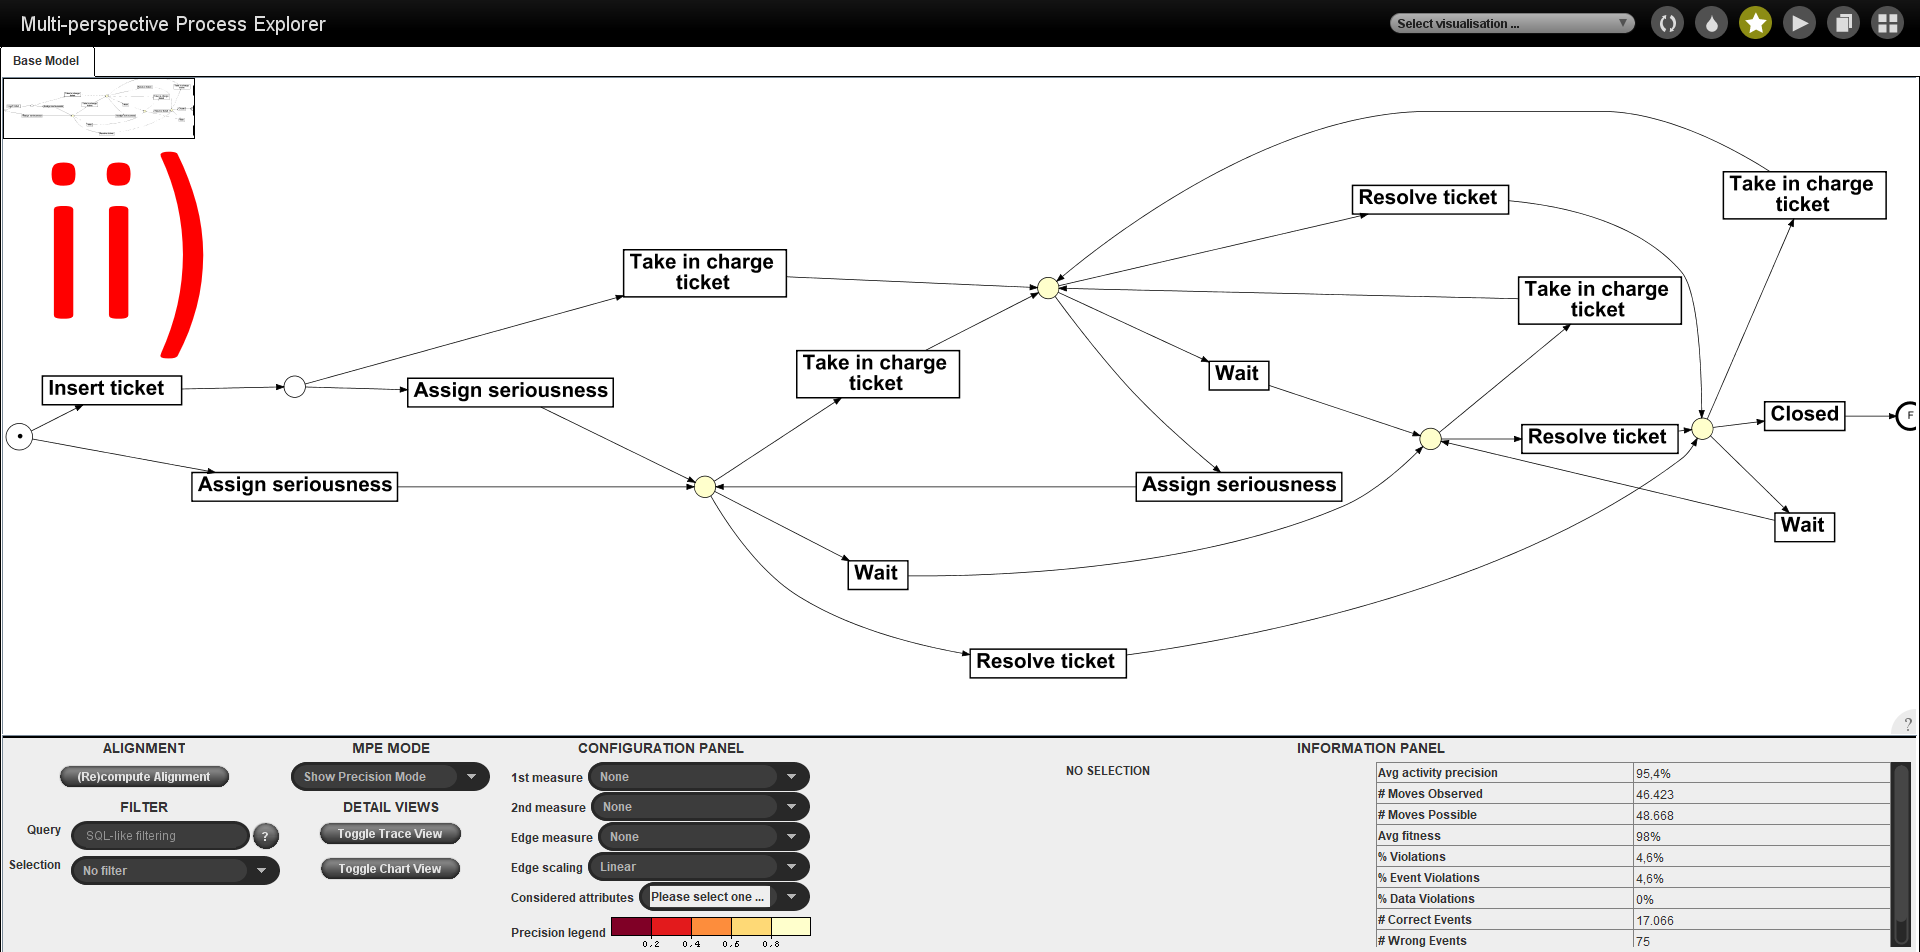
\includegraphics[width=\columnwidth]{Question_2/img/ProM_b_region_ii_PRE.png}\\
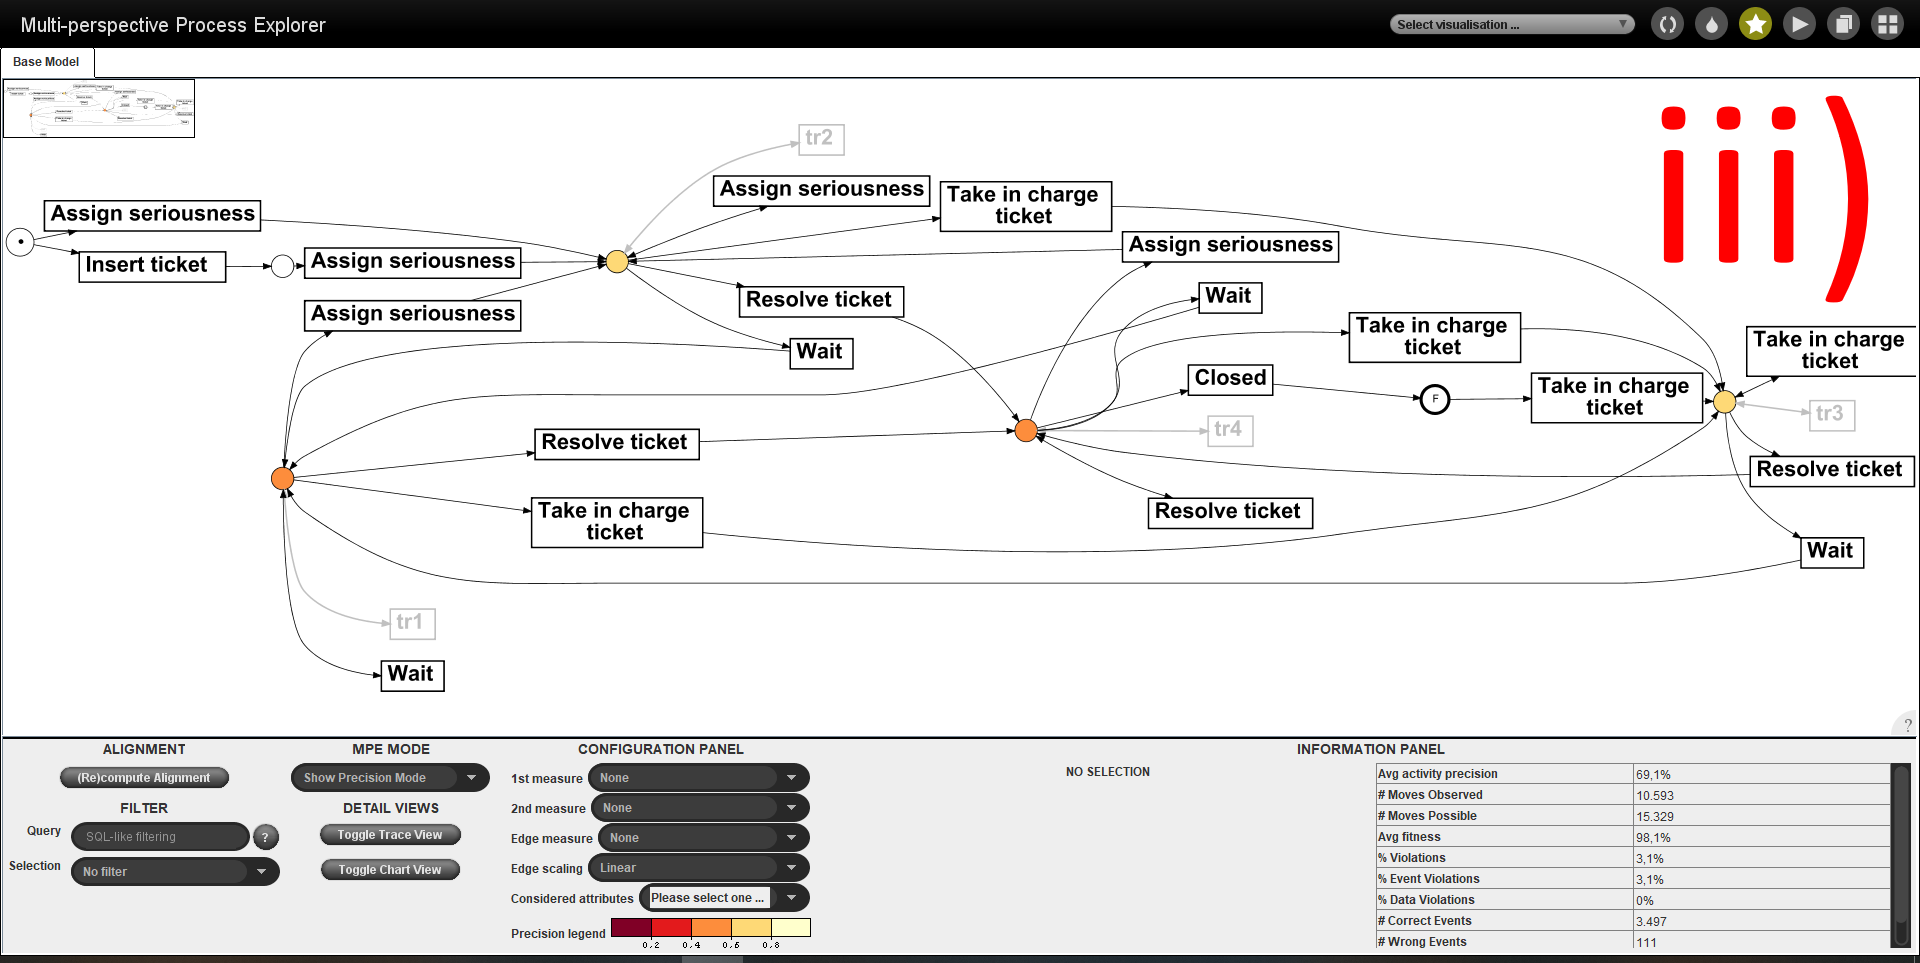
\includegraphics[width=\columnwidth]{Question_2/img/ProM_b_region_iii_POST.png}\\
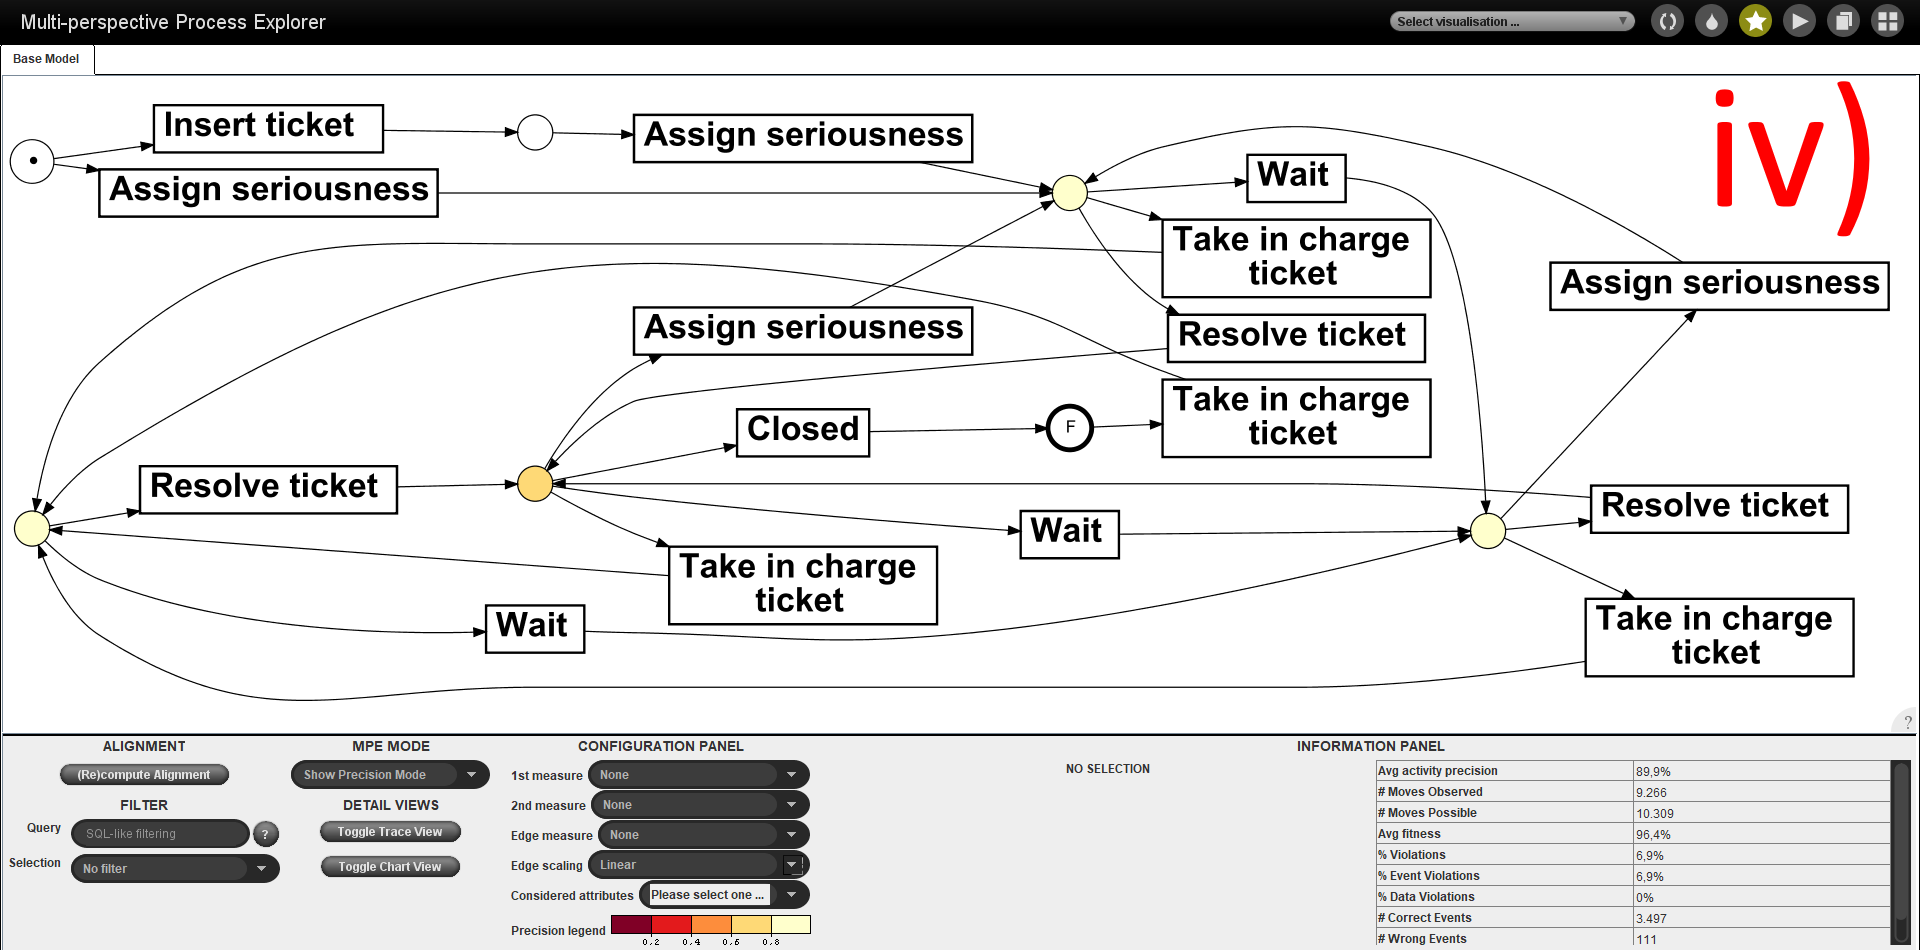
\includegraphics[width=\columnwidth]{Question_2/img/ProM_b_region_iv_POST.png}\\
\subsection*{Question 2(b)3}
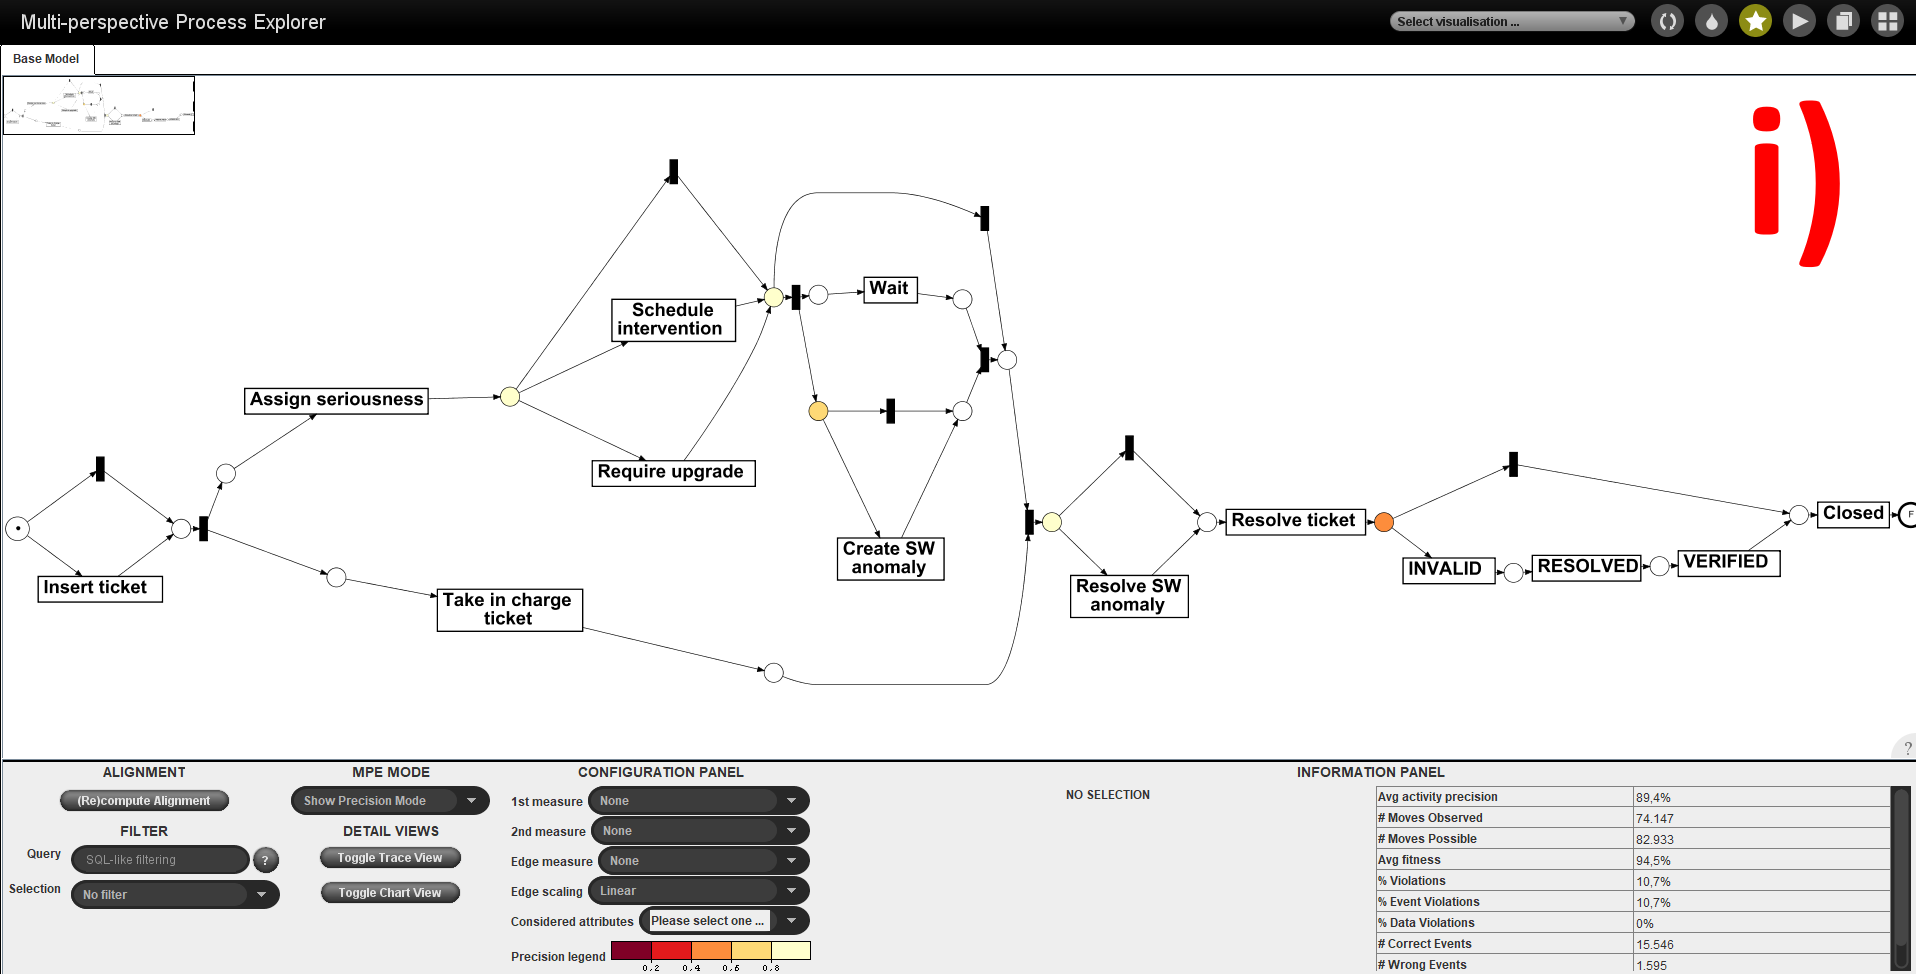
\includegraphics[width=\columnwidth]{Question_2/img/ProM_b_inductive_PRE_i.png}\\
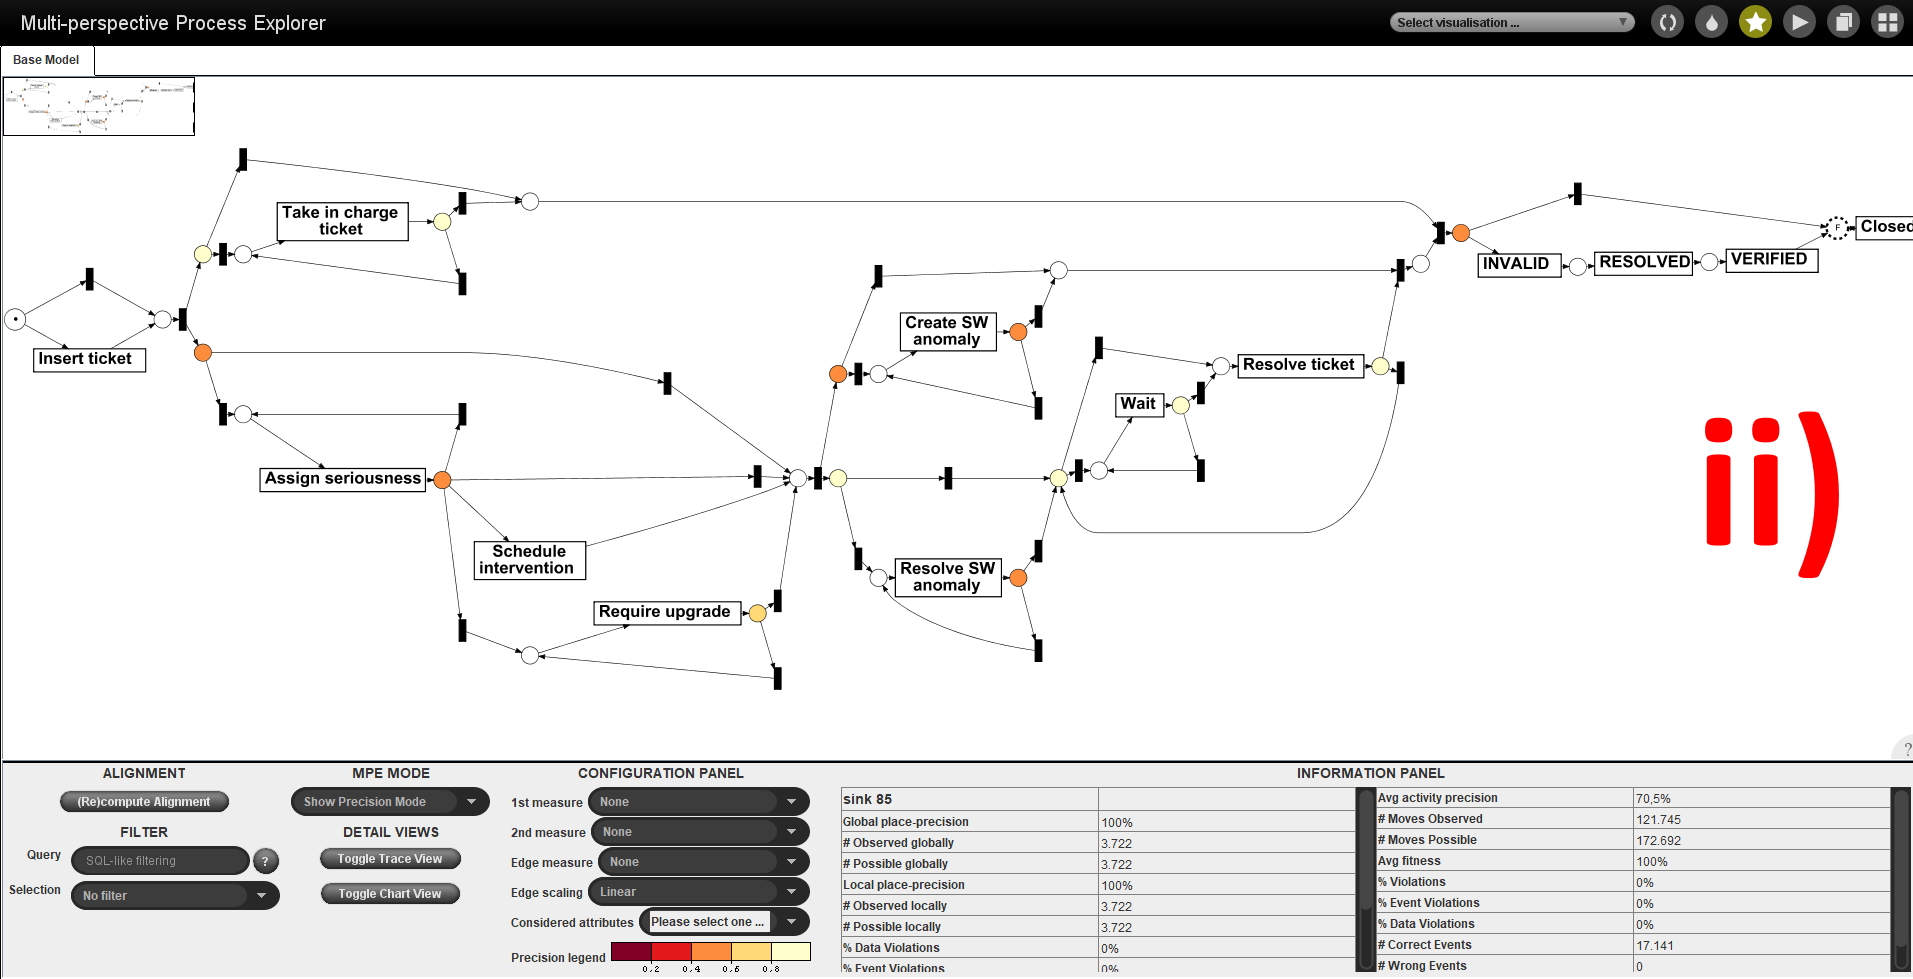
\includegraphics[width=\columnwidth]{Question_2/img/ProM_b_inductive_PRE_ii.png}\\
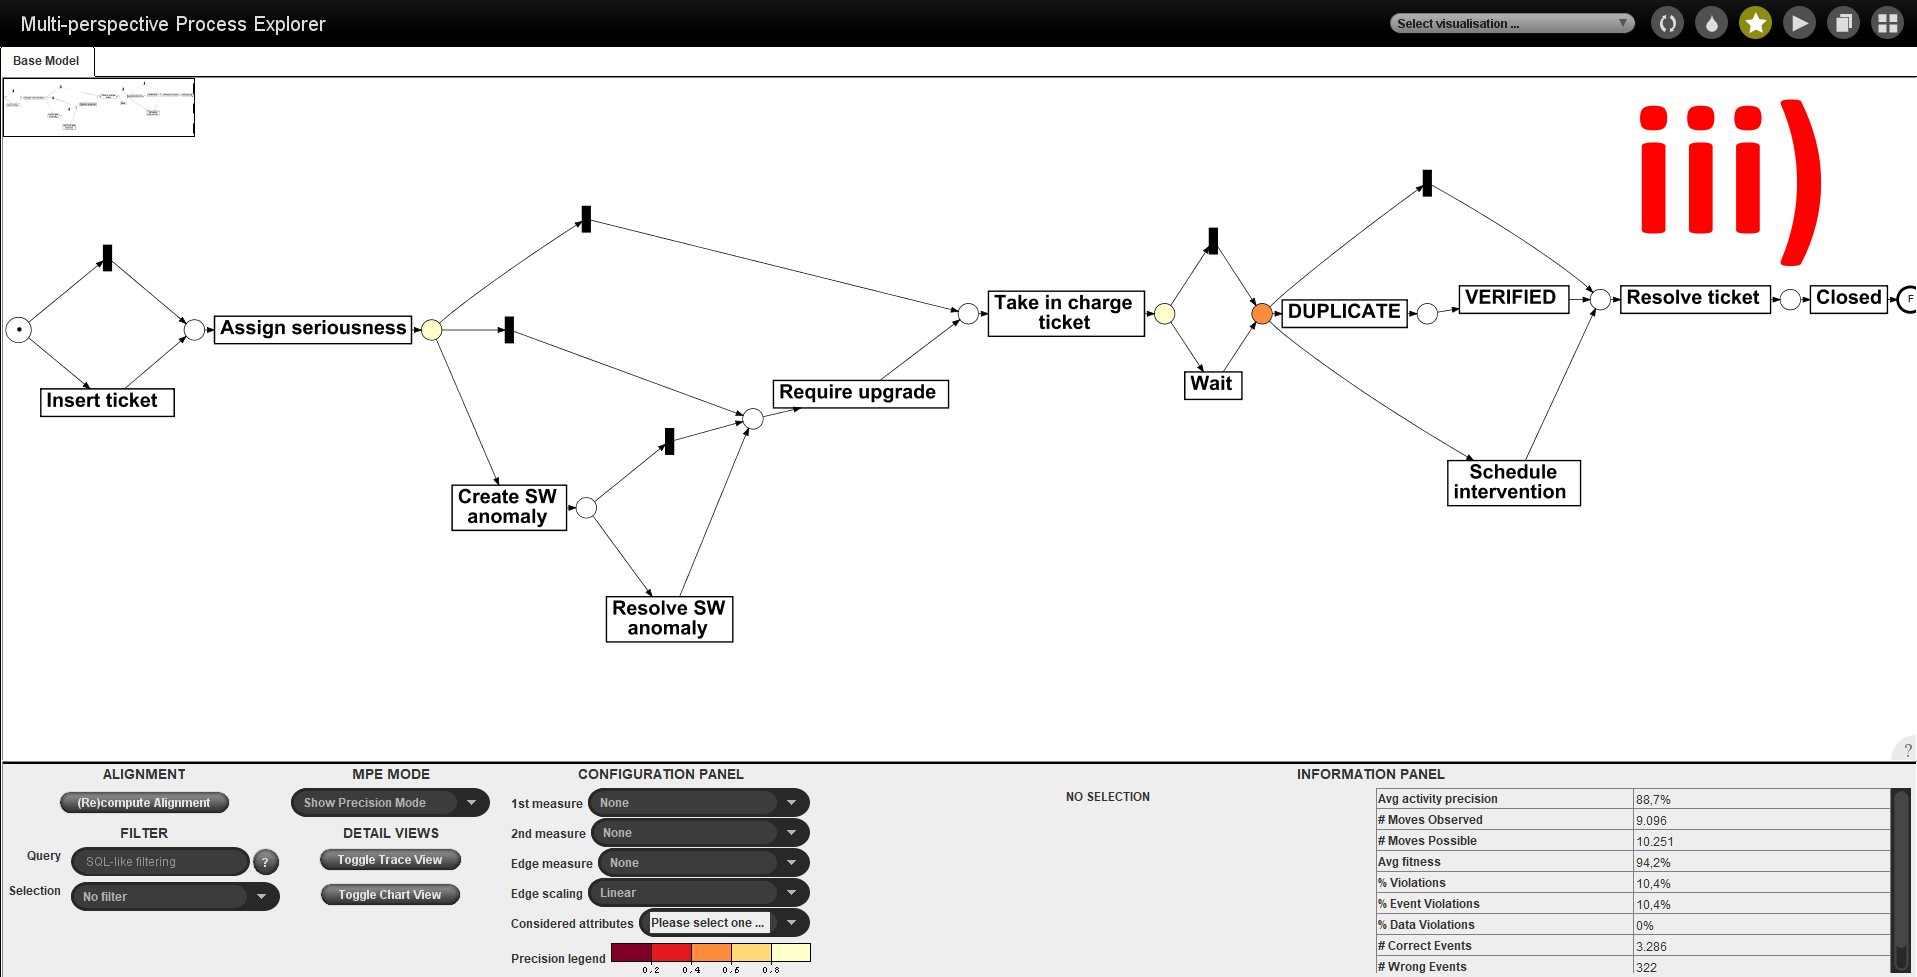
\includegraphics[width=\columnwidth]{Question_2/img/ProM_b_inductive_POST_iii.png}\\
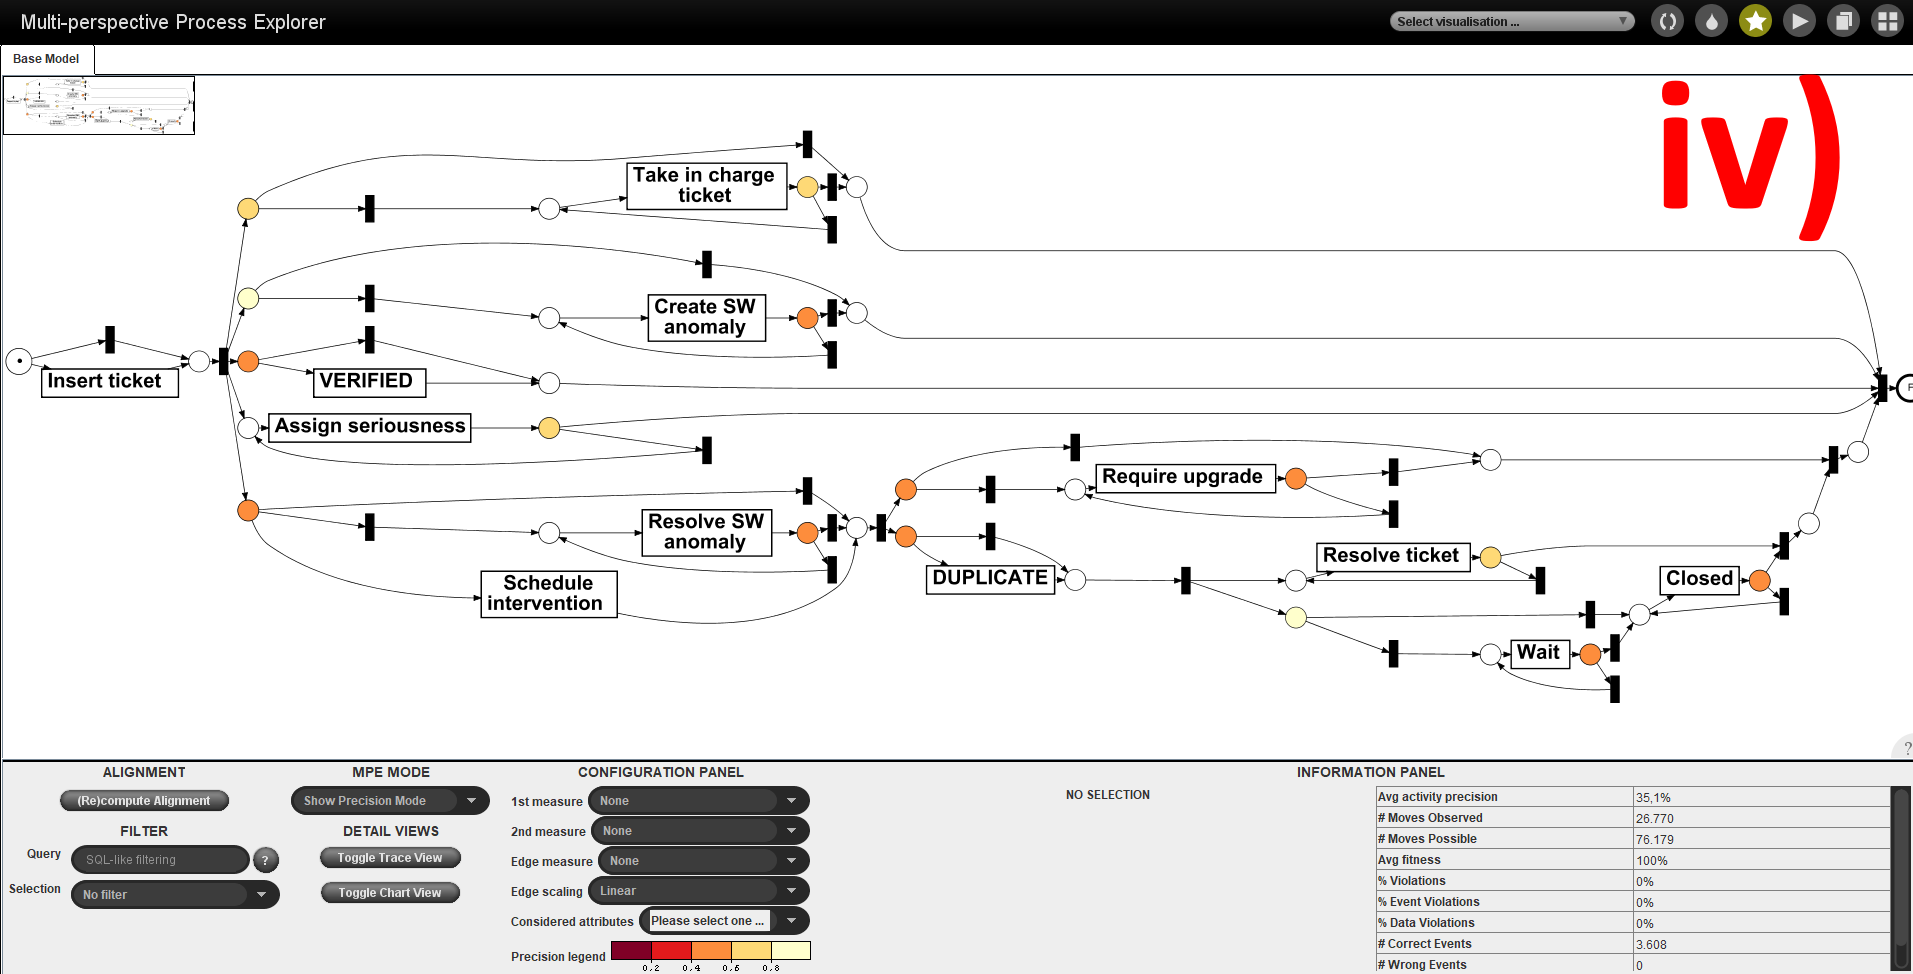
\includegraphics[width=\columnwidth]{Question_2/img/ProM_b_inductive_POST_iv.png}\\
\subsection*{Question 4(b) Decision Tree description:}
\lstinputlisting{Question_4/other/decision-tree-description.txt}
\subsection*{Question 4(b) Decision Tree simplified:}
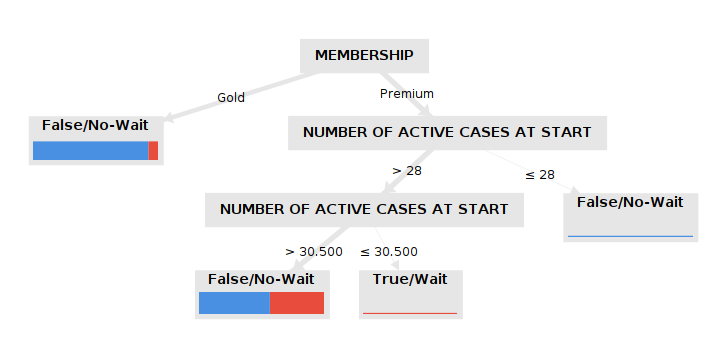
\includegraphics[width=0.75\columnwidth]{Question_4/img/RapidMiner_b_Decision_Tree_simplified.png}

\end{document}